\documentclass[hyperref]{ctexart}
\usepackage{anyfontsize}
%\usepackage[UTF8]{ctex}
%\usepackage{xeCJK}
%\setCJKmainfont{SimSun}
\usepackage{fancyhdr}
\pagestyle{plain}
%\usepackage{hyperref}%书签跳转
\hypersetup{hidelinks}%去掉红框框
\usepackage[section]{placeins}%图片
\usepackage{listings} 
\usepackage{xcolor}
\usepackage{amsmath}
\usepackage{booktabs}
\title{天线编程作业}
\author{陈传升}

\begin{document}
\maketitle
\newpage
\begin{abstract}
	共计五个编程题目, 均在各自章节后附上matlab源代码. 插图均采用eps格式的矢量图,放大观察不失真. PDF采用 \LaTeX 编写, 书签可直接跳转, 方便查看. 
	\textit{注: 由于能力有限,本报告中所有的方向图, 均为归一化非dB形式的功率方向图. }
\end{abstract}
\tableofcontents


\include{dipole}
\include{loop}



\section{Two-Element Array}
\subsection{要求}
\noindent 根据方向图乘积定理,画出不同组态的电偶极子元天线二元阵的方向图
\begin{align*}
&d=\lambda/4, \beta=0\\
&d=\lambda/4, \beta=\pi/2\\
&d=\lambda/2, \beta=0\\
&d=\lambda/2, \beta=\pi\\
&d=\lambda/2, \beta=\pi/2\\
\end{align*}	

\subsection{原理及推导}
根据电偶极子的远场特性,将其z向排阵
\begin{equation}
EF=E_\theta=j\eta\dfrac{kI_0le^{-jkr}}{4\pi r}\cos\theta
\end{equation}
\begin{equation}
(AF)_n=\cos\left[\dfrac{1}{2}(kd\cos\theta+\beta)\right]
\end{equation}
\begin{equation*}
TF=EF\times AF
\end{equation*}
归一化之后常数项没有任何影响,所以
\begin{equation}
E_{total}\simeq \cos\theta\cos\left[\dfrac{1}{2}(kd\cos\theta+\beta)\right]
\end{equation}
\subsection{结果与分析}
如图\ref{fig:2element}所示, 与教材上的结果相符合. 
\begin{figure}[!ht]
	\centering
	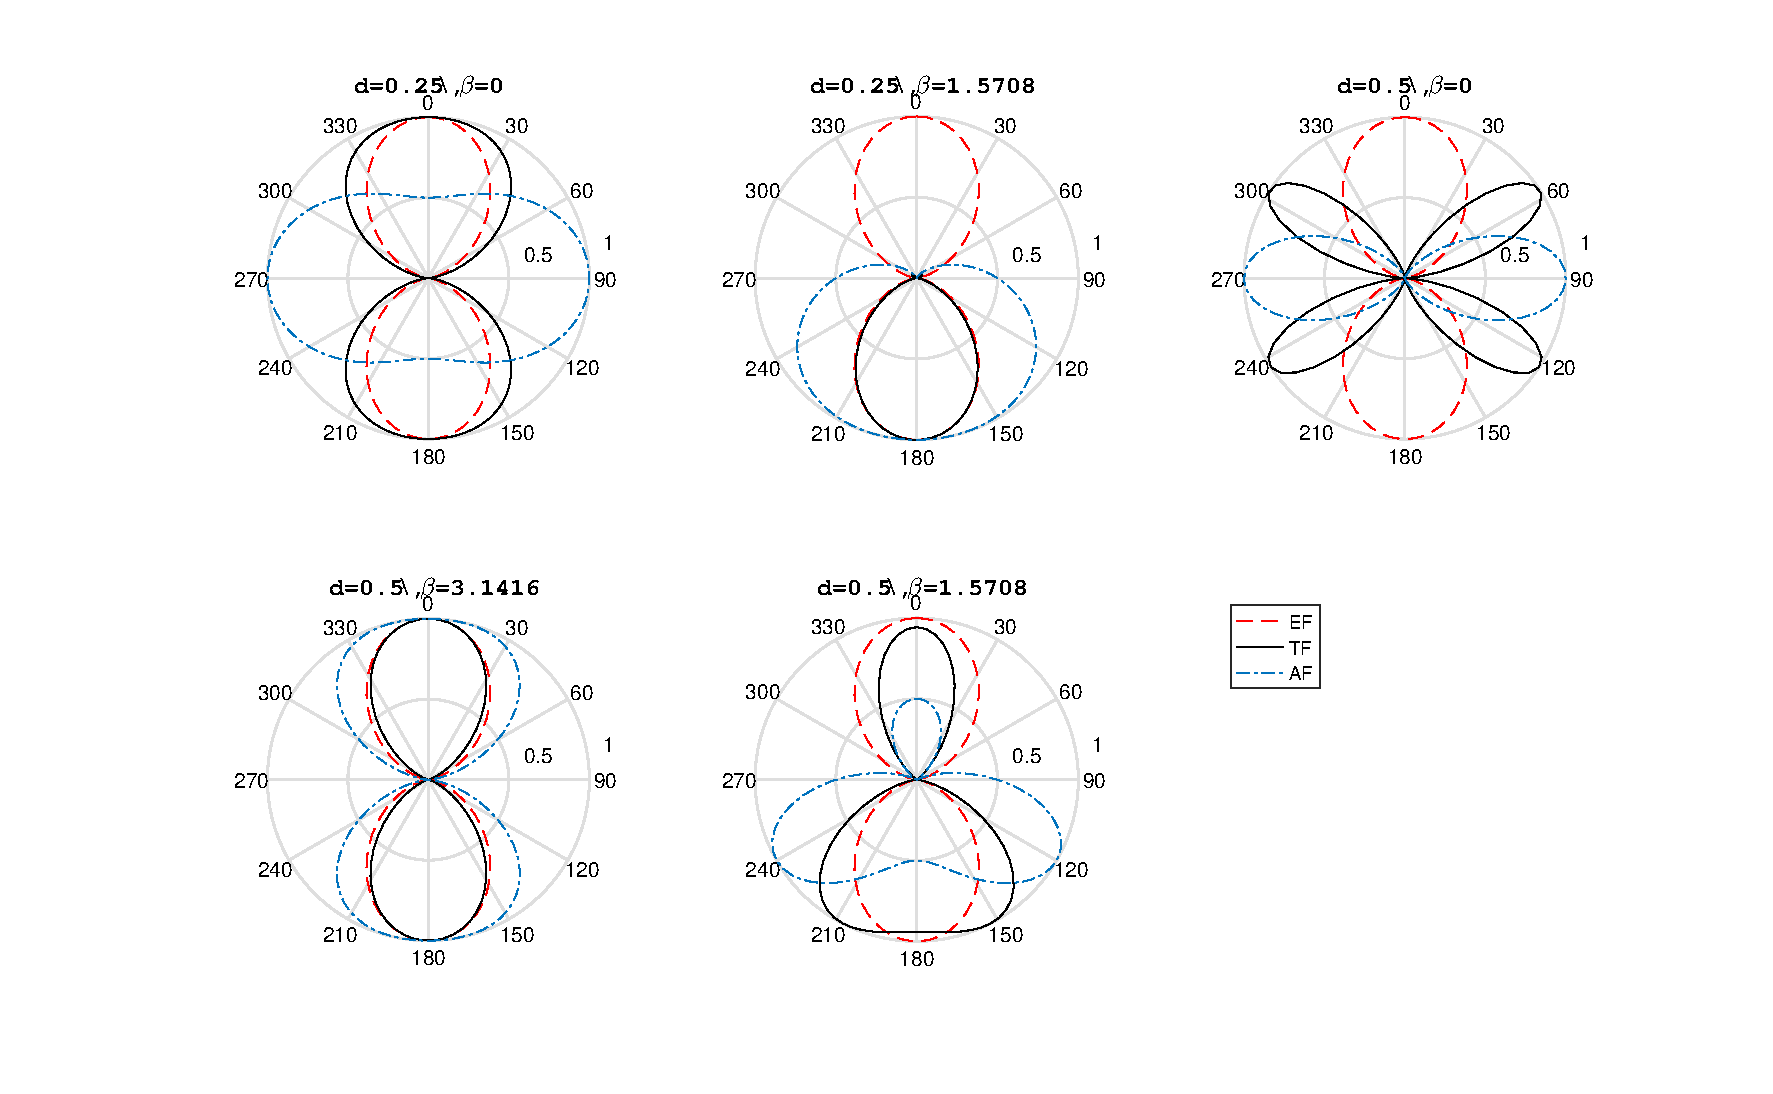
\includegraphics[width=\textwidth]{array2element.eps}
	\caption{$TF=EF\times AF$} \label{fig:2element}
\end{figure}
\newpage
\subsection{程序}
\noindent \textbf{主程序}
\begin{lstlisting}[language={matlab},keywordstyle=\color{blue!70},commentstyle=\color{red!50!green!50!blue!50},frame=shadowbox, rulesepcolor=\color{red!20!green!20!blue!20}] 
clear
close all
d=[0.25 0.25 0.5 0.5 0.5];
beta=[ 0 0.5*pi 0 pi 0.5*pi];
for i=1:5
subplot(2,3,i)
Fun_2array(d(i),beta(i))
end
subplot(2,3,6)
plot(0,0,'r--');hold on
plot(0,0,'k');hold on
plot(0,0,'-.);
axis off
legend('EF','TF','AF','Location','northwest')
\end{lstlisting}
\noindent \textbf{子函数}
\begin{lstlisting}[language={matlab},keywordstyle=\color{blue!70},commentstyle=\color{red!50!green!50!blue!50},frame=shadowbox, rulesepcolor=\color{red!20!green!20!blue!20}] 
function Fun_2array(d,beta)
%d lamda
%beta rad
%phi=kdcos(theta)+beta ??
%?????????????????????????????
theta=linspace(0,2*pi,100);
phi=2*pi*d*cos(theta)+beta;
% EF=abs(cos(theta));         %only E
% AF=abs(cos(0.5*phi));       %only E
EF=cos(theta).^2;         %power
AF=cos(0.5*phi).^2;       %power
TF=AF.*EF;
TF=TF/max(TF);
polar (theta,EF,'r--');hold on
polar(theta,TF,'k');hold on
polar(theta,AF,'-.');
view(90,-90)
% legend('EF','TF','AF','Location','northeastoutside')
titlename=strcat('d=',num2str(d),'\lambda',',', '\beta
=',num2str(beta));
title(titlename,'Fontname','TimeNewsRoman','Fontsize',
12)
end
\end{lstlisting}

\section{Nouniform Amplitude}
\subsection{要求}
\noindent 比较几种不同幅度激励的等间距($\lambda/4$)10元边射阵方向图.并分别计算他们的第一旁瓣电平和HPBW. 


1.均匀分布  $a_1=a_2=a_3=a_4=a_5=1$

2.二项式分布 $a_1=126, a_2=84, a_3=36, a_4=9, a_5=1$

3. Dolph-Tschebyscheff分布$a_1=2.798, a_2=2.496, a_3=1.974, a_4=1.357, a_5=1$
\\

\noindent 选做:

1.根据第4题1中的计算的10元均匀分布情形,用编程数据计算HPBW和D0,并与Tschebyscheff阵的经验预估值(6.8.3-C部分)比较

2.若选单元为沿z轴放置的元天线,根据图乘法画出总方向图
\\
\noindent 提示:电偶极子元天线方向图(垂直于z轴放置 )
\begin{equation}
EF=E_\theta=j\eta\dfrac{kI_0le^{-jkr}}{4\pi r}\cos\theta
\end{equation}


\subsection{原理及推导}
对于N元阵,其阵因子
\begin{equation}
AF_{2M}(even)=\sum_{n=1}^{M}a_n\cos\left[\left(2n-1\right)u\right].
\end{equation}
\begin{equation}
AF_{2M}(odd)=\sum_{n=1}^{M+1}a_n\cos\left[2\left(n-1\right)u\right].
\end{equation}
其中
\begin{equation}
u=\frac{\pi d}{\lambda}\cos\theta
\end{equation}

考虑单元因子的情况下, 根据图乘法, $TF=AF\times EF$,编程也很容易计算.  

\subsection{结果与分析}
\subsubsection{不同幅度激励的等间距10元边射阵}

\paragraph{HPBW}

如表\ref{tab:hpbw}所示, 发现二项式激励的HPBW和等幅激励相比变胖了很多,而切比雪夫激励的HPBW则变化很小,有良好的方向性,可以认为是最优的激励方式.
\begin{table}[!ht]
	\centering
	\begin{tabular}{c|ccc}
		\toprule
		激励方式&等幅激励&二项式激励&切比雪夫激励\\
		\midrule
		HPBW /$^\circ$&24.3360  &48.8160 &  29.5200\\
		\bottomrule
	\end{tabular}
	\caption{不同激励方式的HPBW} \label{tab:hpbw}
\end{table}

\paragraph{第一旁瓣电平(功率)}
如图\ref{fig:LobeValue}所示,二项式激励不存在旁瓣,而切比雪夫激励的旁瓣电平远远小于等幅激励的第一旁瓣电平.

\textit{注:图中标注的点,并非是第一旁瓣电平,而是第一旁瓣的归一化辐射功率(非dB),二者的物理本质是相同的,故不做区分. }
\begin{figure}[!ht]
	\centering
	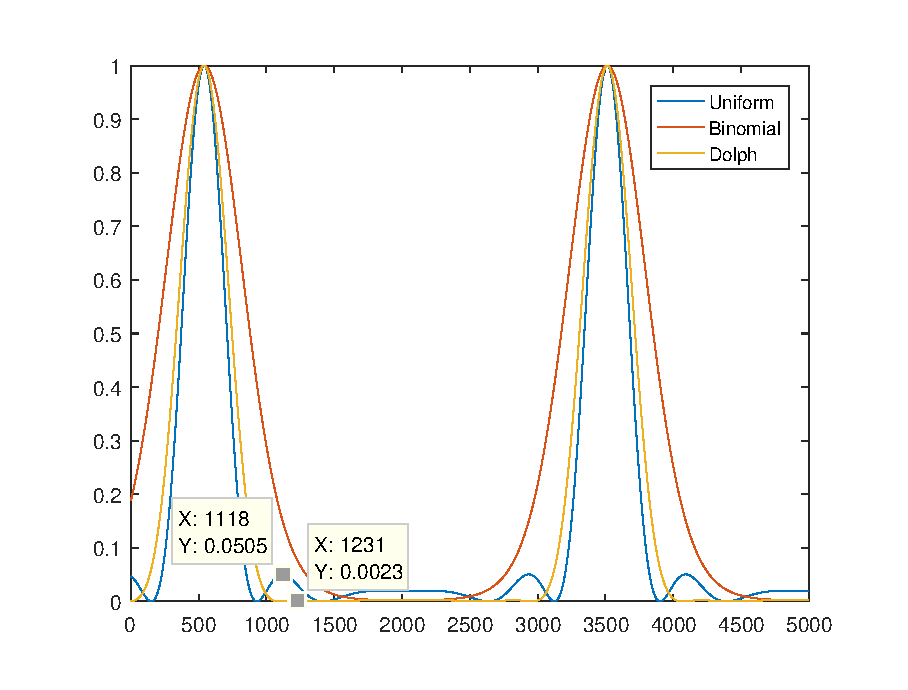
\includegraphics[width=10cm]{TenEle_without_EF_lobeValue.eps}
	\caption{第一旁瓣功率} \label{fig:LobeValue}
\end{figure}


\paragraph{方向图}


根据图\ref{fig:10elenoEF}所示,放大观察如图\ref{fig:10elenoEF_fangda}.

容易发现, 二项式分布的激励,理论上没有任何旁瓣,但是HPBW明显增加.而Dolph-Tschebyscheff分布的激励,其旁瓣电平很小,而且HPBW也很窄,可以认为是最优分布. 
\begin{figure}[!ht]
	\begin{minipage}[t]{0.35\linewidth}
		\centering
		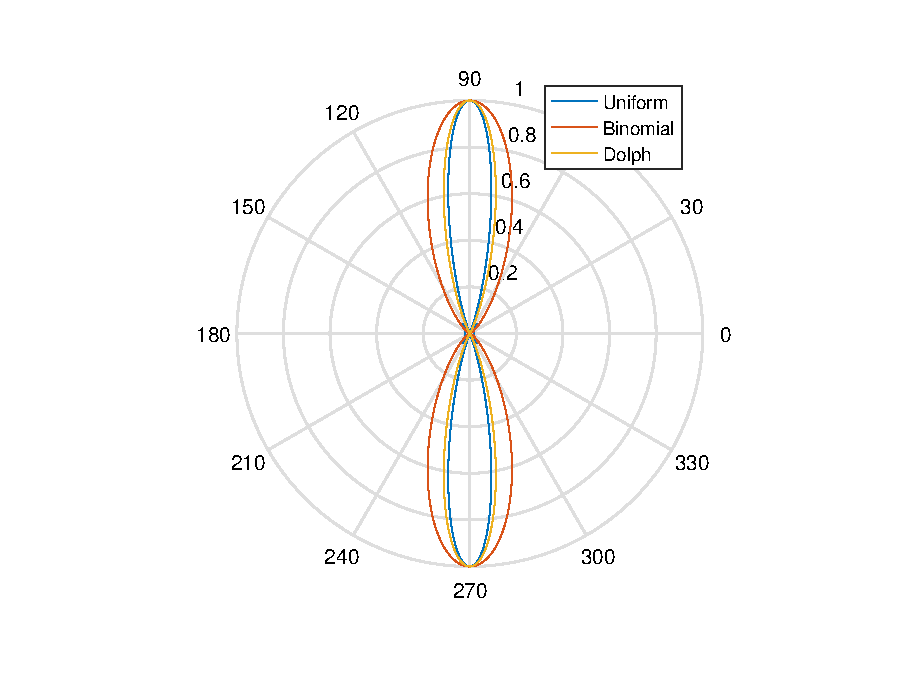
\includegraphics[height=5.5cm,width=7.5cm]{TenEle_without_EF.eps}
		\caption{Pattern without EF}\label{fig:10elenoEF}
	\end{minipage}%
	\hfill
	\begin{minipage}[t]{0.5\linewidth}
		\centering
		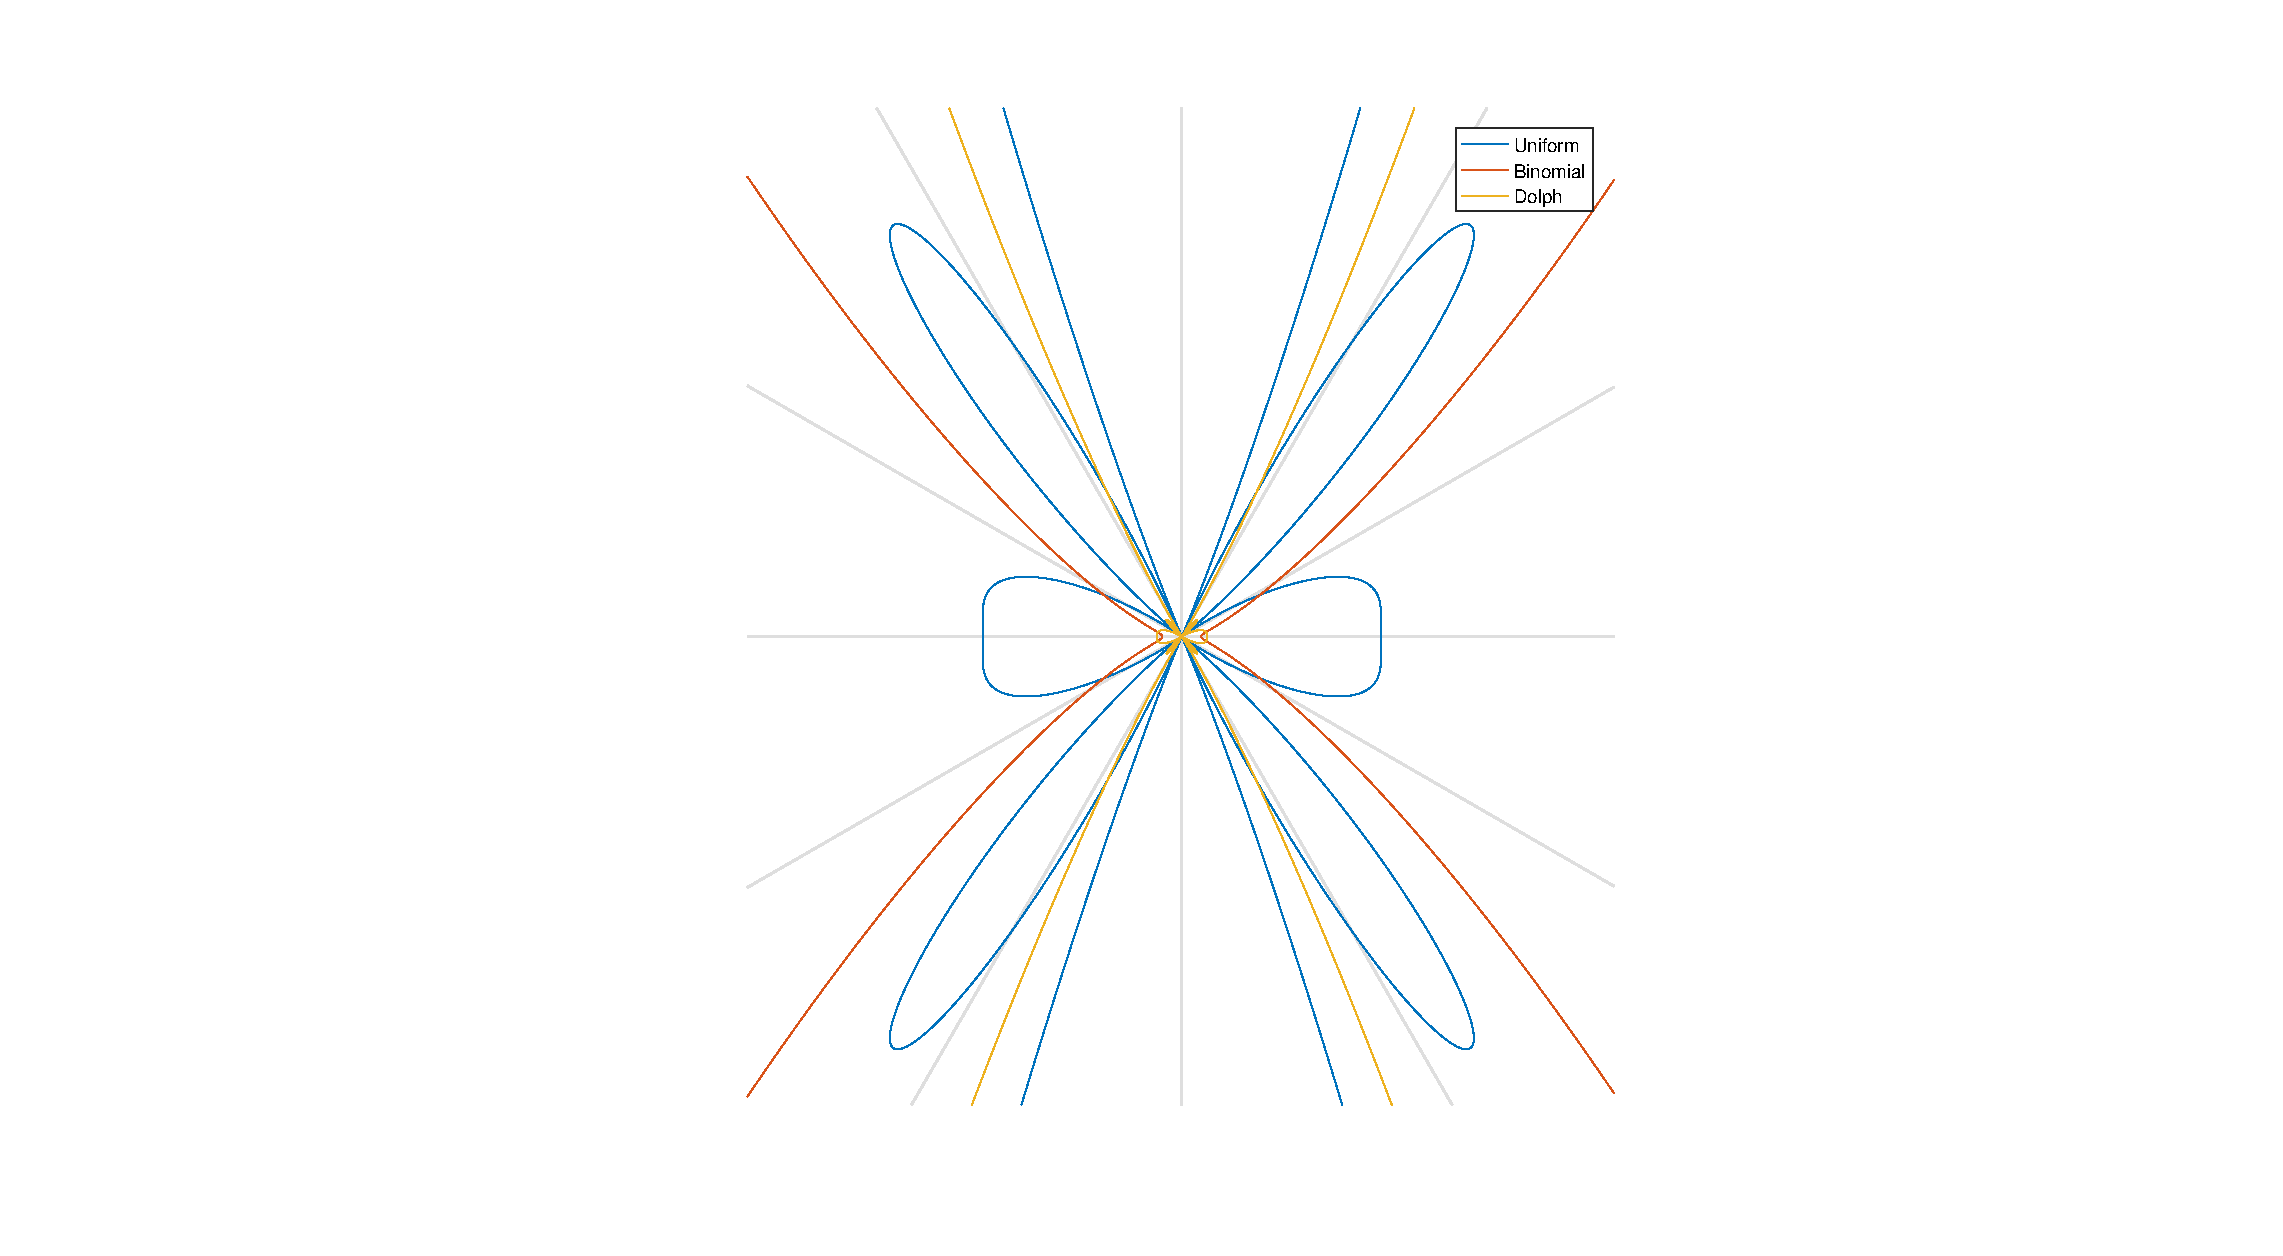
\includegraphics[height=5.5cm,width=7.5cm]{TenEle_without_EF_fangda.eps}
		\caption{放大图}\label{fig:10elenoEF_fangda}
		
	\end{minipage}
\end{figure}


\subsubsection{选做:考虑单元因子的边射阵方向图}
\begin{figure}[!ht]
	\begin{minipage}[t]{0.35\linewidth}
		\centering
		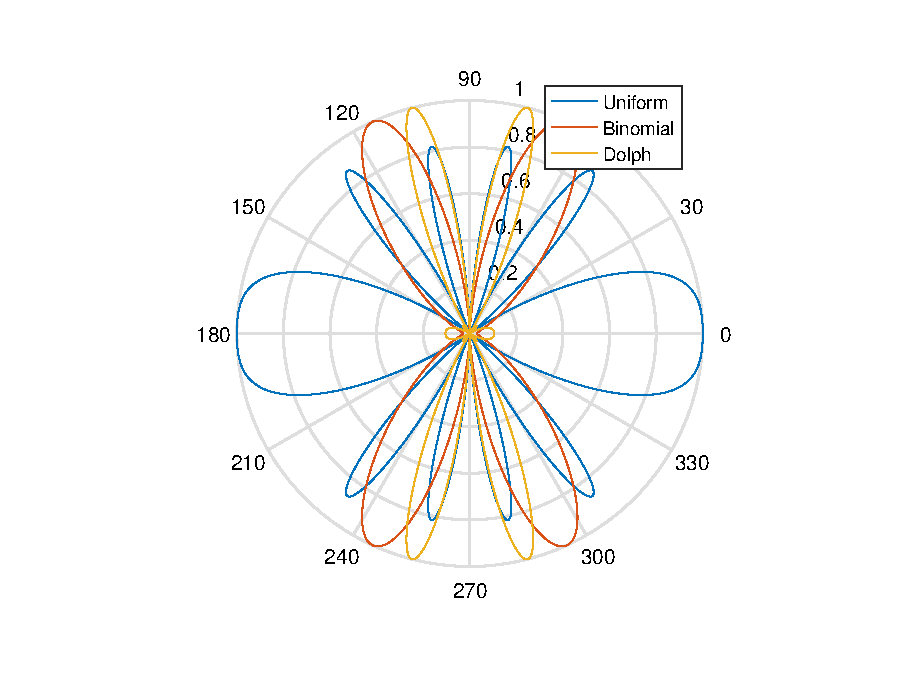
\includegraphics[height=5.5cm,width=7.5cm]{TenEle_with_EF.eps}
		\caption{Pattern with EF}
	\end{minipage}%
	\hfill
	\begin{minipage}[t]{0.5\linewidth}
		\centering
		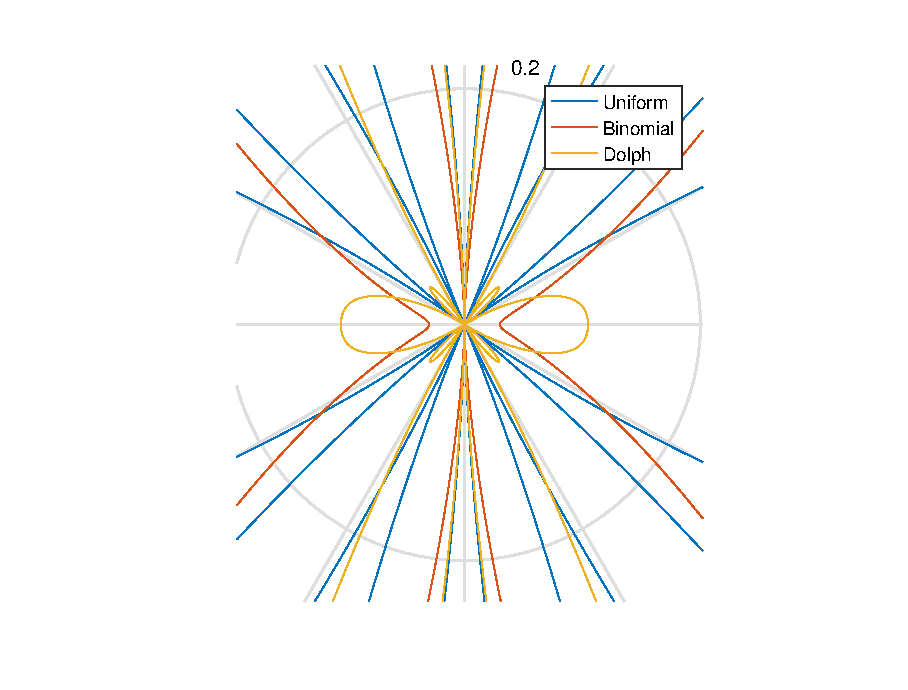
\includegraphics[height=5.5cm,width=7.5cm]{TenEle_with_EF_fangda.eps}
		\caption{放大图}
		
	\end{minipage}\label{fig:10eleEF}
\end{figure}

\subsection{程序}
\noindent \textbf{主程序}
\begin{lstlisting}[language={matlab},keywordstyle=\color{blue!70},commentstyle=\color{red!50!green!50!blue!50},frame=shadowbox, rulesepcolor=\color{red!20!green!20!blue!20}]clear
close all

a1=[1 1 1 1 1 1 1 1 1 1];
a2=[126 84 36 9 1 0 0 0 0 0];
a3=[2.798 2.496 1.974 1.357 1 0 0 0 0 0];
theta=linspace(1,2*pi,5000);

d=0.25;
[AF1,HPBW1]=Fun_TenElement_array(a1,d);
[AF2,HPBW2]=Fun_TenElement_array(a2,d);
[AF3,HPBW3]=Fun_TenElement_array(a3,d);

polar(theta, AF1/max(AF1));hold on 
polar(theta, AF2/max(AF2));hold on 
polar(theta, AF3/max(AF3));hold on 
legend('Uniform','Binomial','Dolph')
[HPBW1,HPBW2,HPBW3]
figure
x=1:5000;
plot(x,AF1/max(AF1));hold on
plot(x,AF2/max(AF2));hold on
plot(x,AF3/max(AF3));hold on
legend('Uniform','Binomial','Dolph')
%Solve 3dB BandWidth


figure 
Fun_TenElement_array_with_EF(a1,d)
hold on 
Fun_TenElement_array_with_EF(a2,d)
hold on 
Fun_TenElement_array_with_EF(a3,d)
hold on 
legend('Uniform','Binomial','Dolph')
%legend('1','2','che')





\end{lstlisting}

\noindent \textbf{子函数不考虑EF}
\begin{lstlisting}[language={matlab},keywordstyle=\color{blue!70},commentstyle=\color{red!50!green!50!blue!50},frame=shadowbox, rulesepcolor=\color{red!20!green!20!blue!20}] 
function [AF,BeamWidth_3dB]=Fun_TenElement_array(a,d)
%Output_1 is AF array,stepnum is 5000,form 0to2pi
%Outpuit_2 is BeamWidth_3dB,

n=length(a);
flag=(mod(n,2)==1); % 1 is odd, 0 is even
AF=0;
theta=linspace(1,2*pi,5000);
u=pi*d*cos(theta);
if flag==0

for i=1:n/2
AF=AF+a(i)*cos((2*i-1)*u);
end

else %odd

for i=1:fix(n/2)
AF=AF+cos(2*(i-1)*u);
end

end
AF=AF.^2;   %POWER

%solve 3dB BandWidth
AF_1=AF/max(AF);
dB3=find(AF_1(1:2000)>=0.5);
BeamWidth_3dB=(max(dB3)-min(dB3))/5000*360;

end
\end{lstlisting}

\noindent \textbf{子函数考虑EF}
\begin{lstlisting}[language={matlab},keywordstyle=\color{blue!70},commentstyle=\color{red!50!green!50!blue!50},frame=shadowbox, rulesepcolor=\color{red!20!green!20!blue!20}]
function Fun_TenElement_array_with_EF(a,d)

n=length(a);
flag=(mod(n,2)==1); % 1 is odd, 0 is even
AF=0;
theta=linspace(1,2*pi,5000);


u=pi*d*cos(theta);
if flag==0

for i=1:n/2
AF=AF+a(i)*cos((2*i-1)*u);
end

else %odd

for i=1:fix(n/2)
AF=AF+cos(2*(i-1)*u);
end

end

AF=AF.^2;
TF=cos(theta).^2.*AF;
polar(theta, TF/max(TF));
hold on 

end
\end{lstlisting}

\section{Helical Antenna}
\subsection{要求}
\noindent 
根据轴向模螺旋天线驻波(普通端射模式)的方向图计算公式
\begin{equation}
E=\sin\left(\frac{\pi}{2N}\right)\cos\theta\dfrac{\sin\left[\left(N/2\right)\psi\right]}{\sin\left[\psi/2\right]}.
\end{equation}
其中
\begin{equation}
\psi=k_0\left(S\cos\theta-\frac{L_0}{p}\right), p=\frac{L_0/\lambda_0}{S/\lambda_0 +1}.
\end{equation}
画出一个沿z轴放置、$N=8$圈、螺距$S=\lambda/4$、单圈线长$L_0=\lambda$的轴向模螺旋天线的竖直平面(x=0)方向图。

\noindent 选做:

1.根据天线的对称性,利用编程数据计算$D_0$,并与经验公式$D_0\simeq15n\dfrac{c^2S}{\lambda_0^3}$
的结果进行比较


\subsection{原理及推导}
分析方向图计算公式发现$E\sim\left(N,S,L,\theta\right)$. 在编程的时候输入参量$S,L$均是以$\lambda$为单位, 所以$\psi$可以化简如下
\begin{equation}
\psi=2\pi\left(S\cos\theta-\frac{L}{p}\right), p=\frac{L}{S+1}.
\end{equation}
故编程时写作
\begin{lstlisting}[language={matlab},keywordstyle=\color{blue!70},commentstyle=\color{red!50!green!50!blue!50},frame=shadowbox, rulesepcolor=\color{red!20!green!20!blue!20}] 
p=L/(S+1);
psi=2*pi*(S*cos(theta)-L/p);
A=sin(pi/2/N);
B=cos(theta);
C=sin(N/2*psi)./sin(psi/2);
E=A.*B.*C;
Power=E.^2;
\end{lstlisting}

计算方向性的经验公式, 约去$\lambda_0$后, 得到
\begin{equation}
D=15Nc^2 S
\end{equation}
\subsection{结果与分析}
\subsubsection{方向图及$D_0$}
归一化,非dB的辐射功率方向图如图\ref{fig:HelixP}所示, 为了观察后瓣情况, 放大图如图\ref{fig:HelixP_fangda}. 
\begin{figure}[!ht]
	%\small
	\centering
	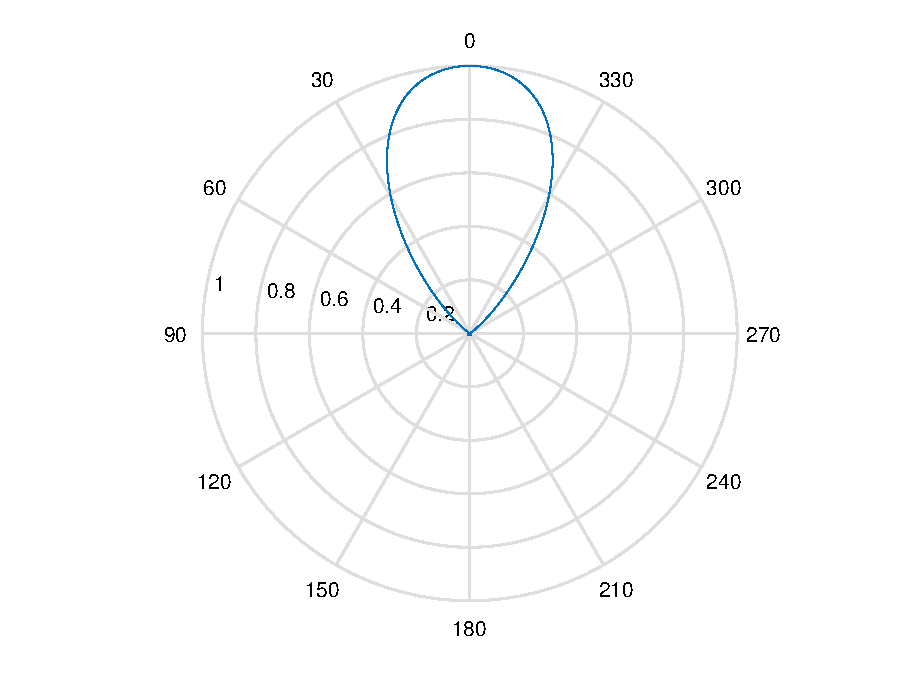
\includegraphics[width=10cm]{HelixPattern.eps}
	\caption{Helical Antenna Pattern} \label{fig:HelixP}
\end{figure}

\begin{figure}[!ht]
	%\small
	\centering
	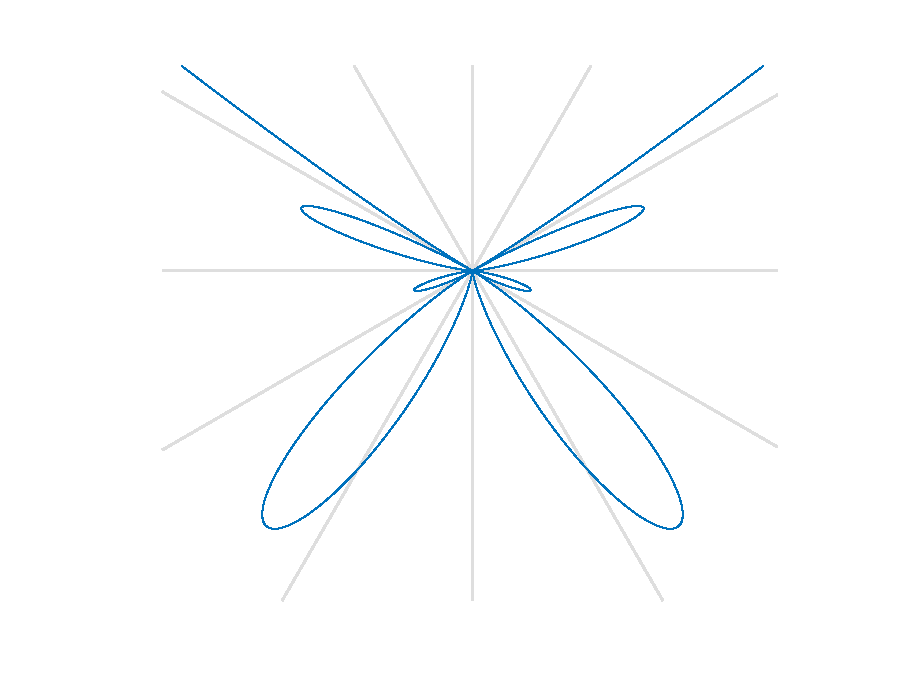
\includegraphics[width=10cm]{HelixPattern_fangda.eps}
	\caption{放大图} \label{fig:HelixP_fangda}
\end{figure}




\subsubsection{选做:与经验公式的对比}
经验公式计算结果为:
\begin{equation}
D=15Nc^2 S=15N(L^2-S^2) S=28.125.
\end{equation}
所以$D(dB)=14.49$.


编程计算的结果为$D_0=12.40$
\subsection{程序}
\noindent \textbf{主程序}
\begin{lstlisting}[language={matlab},keywordstyle=\color{blue!70},commentstyle=\color{red!50!green!50!blue!50},frame=shadowbox, rulesepcolor=\color{red!20!green!20!blue!20}] 
clear
close all
N=8;S=0.25;L=1;
Fun_Helix(N,S,L)
%Compare equation
clear
syms theta
N=8;S=0.25;L=1;
p=L/(S+1);
psi=2*pi*(S*cos(theta)-L/p);
A=sin(pi/2/N);
B=cos(theta);
C=sin(N/2*psi)/sin(psi/2);
E=A*B*C;
Power=E^2;
PP=cos(theta)*sin(8*pi*(0.25*cos(theta)-1.25))/sin(pi*(0.25*cos(theta)-1.225));
a=vpa(int(2*pi*Power,theta,[0,2*pi]),6)
D=10*log10(a)
% b=int(PP,theta,[0,2*pi])
% vpa(b,6)
% D=4*pi*2.4359/a;

D_exp=10*log10(15*N*(L^2-S^2)*S)



\end{lstlisting}
\noindent \textbf{子函数}
\begin{lstlisting}[language={matlab},keywordstyle=\color{blue!70},commentstyle=\color{red!50!green!50!blue!50},frame=shadowbox, rulesepcolor=\color{red!20!green!20!blue!20}] 
function Fun_Helix(N,S,L)
%Polar Pattern
%Input N,S/Lambda,L0/lambda
%Output D is directivity
theta=linspace(0,2*pi,5000);
p=L/(S+1);
psi=2*pi*(S*cos(theta)-L/p);
A=sin(pi/2/N);
B=cos(theta);
C=sin(N/2*psi)./sin(psi/2);

E=A.*B.*C;
Power=E.^2;
polar(theta,Power/max(Power));
view(-90,90)
% max(E.^2)
% D=max(Power)/mean(Power);
end
\end{lstlisting}
\end{document}